% Section content template for individual Educative lessons
% This file contains the actual content for a specific section
% Generated from Educative API section content

% Section: Requirements for the ATM System
% Section ID: 5777893008605184
% Section Slug: requirements-for-the-atm-system
% Generated: 2025-12-12T15:53:08.800694

In this lesson, we outline the functional and operational requirements for the ATM System. Identifying and understanding requirements is essential to defining the system's scope and ensuring a robust, user-friendly design.
\\
We'll use the notational convention to identify each requirement with a unique label, ``Rn,'' where ``R'' is short for requirement, and ``n'' is a natural number.

\subsection{Requirement collection}\label{l26NQTUTc4yL2-Ol9v6FB}

\begin{itemize}
\item
\protect\phantomsection\label{WnDNUNrHcjMr2W_zvVd3u}
\textbf{R1:} Each user has a single account at the bank that they can access by inserting their card into the ATM.
\item
\protect\phantomsection\label{2nV7XSAoXenSQ5qjFuMrF}
\textbf{R2:} The ATM system consists of the following main components to facilitate user interaction and transaction processing:

\begin{itemize}
\item
\protect\phantomsection\label{jc_AYLO5G2fKus6nk1FCa}
\textbf{Card Reader:} Reads the user's ATM card.
\item
\protect\phantomsection\label{Ba0m8O7erTdBwneKSDTnH}
\textbf{Keypad:} The user can enter their PIN and transaction details.
\item
\protect\phantomsection\label{i4lVxjSAHpx0bIKaUykXm}
\textbf{Screen:} Displays prompts, messages, and transaction information.
\item
\protect\phantomsection\label{NdASWVytHwItwZcNQjyS6}
\textbf{Cash Dispenser:} Dispenses cash to the user for withdrawal transactions.
\item
\protect\phantomsection\label{d6mnhTvv7Dw5cyWS7xZ8M}
\textbf{Printer:} Prints transaction receipts for the user.
\item
\protect\phantomsection\label{C6lowRSxsSfo_-m4vtRK2}
\textbf{Network Infrastructure:} Securely connects the ATM to the bank's central system to process transactions and access account information.
\end{itemize}
\item
\protect\phantomsection\label{AXm91wvUv8Q29LhE8fKae}
\textbf{R3:} The ATM must authenticate users by verifying the PIN entered, ensuring that only authorized customers can access account services.
\item
\protect\phantomsection\label{Vtf1dzSu2NvUQB9UDQqwK}
\textbf{R4:} All transaction options become available only after successfully authentication the card and PIN.
\item
\protect\phantomsection\label{HM0rALpEmI62k7zlLkUb2}
\textbf{R5:} Users may have either or both of the following account types:

\begin{itemize}
\item
\protect\phantomsection\label{ig9kgcweyxztfJjPOF5z0}
Current account
\item
\protect\phantomsection\label{cxsk2-BDfQZ4tIekebDpD}
Savings account
\end{itemize}
\item
\protect\phantomsection\label{jYEjQvw70SaNdgGKkLqUj}
\textbf{R6:} The ATM must allow the following operations for each account type:

\begin{itemize}
\item
\protect\phantomsection\label{My7W_Rnheu6NT8YK_x4_Y}
Balance inquiry
\item
\protect\phantomsection\label{vRWXeICNT5Jo529kKgF5r}
Cash withdrawal
\item
\protect\phantomsection\label{ZHYlK_RW14Sv7ZMI_TDJN}
Funds transfer
\end{itemize}
\item
\protect\phantomsection\label{AQgqVNuC8Do5Zb-zKoWjs}
\textbf{R7:} After completing a transaction, the user should have the option to perform another transaction or end their session and retrieve their card.
\end{itemize}

\begin{figure}[htbp]
 \centering
 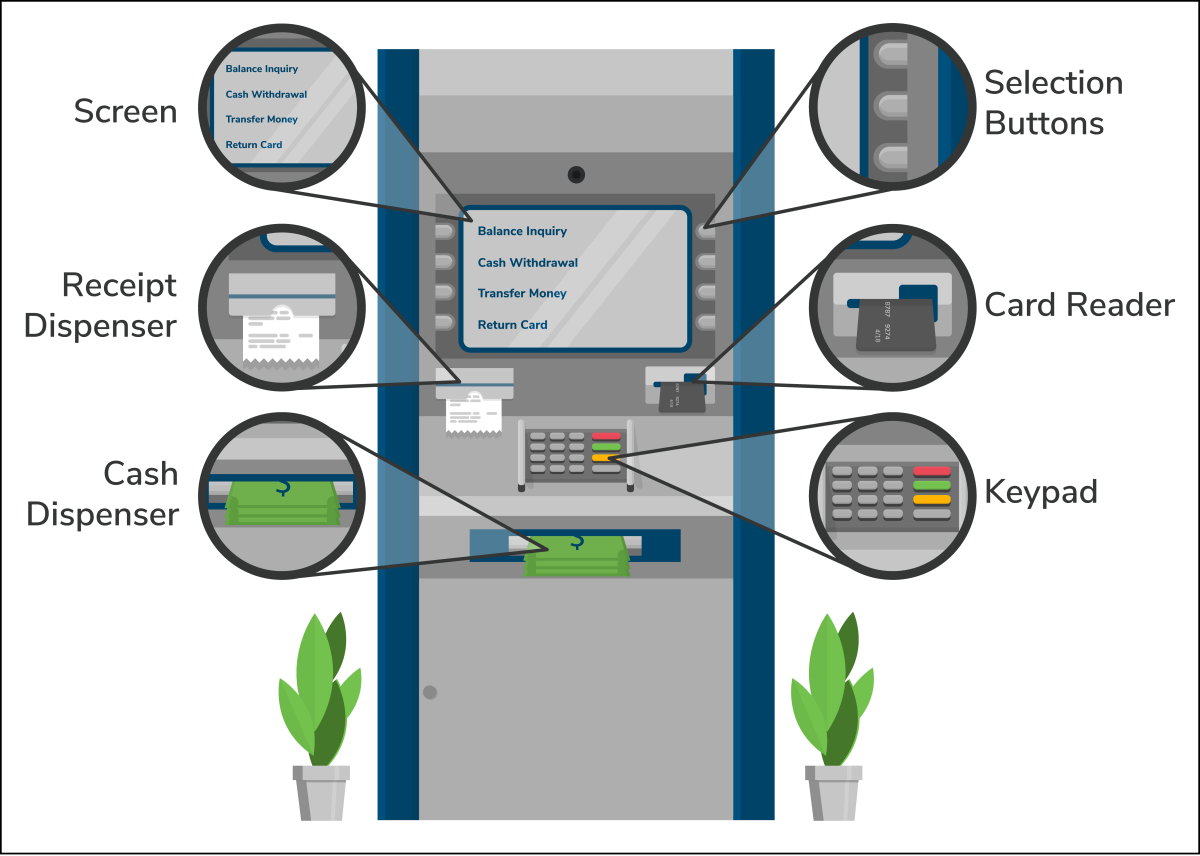
\includegraphics[width=0.5\textwidth]{Images/chapter_16/section_5777893008605184/4827069667344384.png}
 \caption{ATM components}
\end{figure}

We've identified our requirements for the problem. In the next lesson, let's define different use cases of the ATM system.

% End of section content